\chapter{Methodology}
\label{Chapter4}
\lhead{Chapter 4. \emph{Methodology}}
\todo{Describe implementation details}
In this section we are going to discuss the different classes we used to implmeent our solution.

We have used Python's latest version 3.10 on VS Code.
\newpage

\tikzset{class/.style={rectangle, draw=green!60, fill=green!5, very thick, minimum size=20},
method/.style={rectangle, draw=yellow!60, fill=yellow!5, very thick, minimum size=20},
attributes/.style={rectangle, draw=blue!60, fill=blue!5, very thick, minimum size=20},
instance/.style={rectangle, draw=orange!60, fill=orange!5, very thick, minimum size=20}
}

\newpage
\section{Monte Carlo Tree Search} 
In this section, we are first going to dive into an example to explain the Monte Carlo Tree Search algorithm with a simple case. In the second part we are going to generalise it to our problem.

\subsection{Example }
\label{Example}
Let's say we are given a maximisation problem. When starting the game, you have two possible actions $a_1$ and $a_2$ from $S^{0,0}_0$ in the tree $\mathcal{T}$.
Every node is defined like so: $S^{n_i,t_i}_i$ where $n_i$ represents the number of times node $i$ has been visited, $t_i$ the total score of this node.
Furthermore, for every node - we can compute the $UCB1$ value: $UCB1(S^{n_i,t_i}_i)=\bar{V_i} + 2 \sqrt{\frac{\ln N}{n_i}}$ where $\bar{V_i}=\frac{n_i}{t_i}$ represents the average value of the node, $n_i$ the number of times node $i$ has been visited, $N=n_0$ the number of times the root node has been visited/the number of iterations.

Before the first iteration, none node have been visited - $\forall i \in \mathcal{T}, S^{0,0}_{i}$.
\begin{figure}[!ht]
    \centering
        \begin{tikzpicture}[
            root_node/.style={circle, draw=orange!60, fill=orange!5, very thick, minimum size=40},
            visited_node/.style={circle, draw=green!60, fill=green!5, very thick, minimum size=40},
            unvisited_node/.style={circle, draw=gray!60, fill=gray!5, very thick, minimum size=40},
            target_node/.style={circle, draw=green!60, fill=green!5, very thick, minimum size=40},
            ]

            \node[root_node](Root){$S^{0,0}_0$};
            \node[unvisited_node, below left=of Root](S1){$S^{0,0}_1$};
            %\node[target_node, below=of S1, yshift=-1.7cm](Target){};
            \node[unvisited_node, below right=of Root](S2){$S^{0,0}_2$};

            \draw[->] (Root) -- (S1) node[midway, above, xshift=-2mm] {$a_1$};
            \draw[->] (Root) -- (S2) node[midway, above, xshift=2mm] {$a_2$};

            %\draw[->, very thick, decorate, decoration={snake, amplitude=.7mm, segment length=3mm}] (S1) -- (Target);
        \end{tikzpicture}
    \caption{Selection - $I1$}
    \label{fig:Expansion of the tree from the root node}
\end{figure}
At the beginning of $I1$, we then have to choose between these two child nodes (or choose between taking $a_1$ or $a_2$). We then have to calculate the $UCB1$ value for these two nodes and pick the node that maximises the $UCB1$ value (as we are dealing with a maximisation problem).
In Figure \ref{fig:Expansion of the tree from the root node}, neither of these have been visited yet so $USB(S^{0,0}_1)=UCB1(S^{0,0}_2)=\infty$. Hence we decide to choose randomly $S^{0,0}_1$.

$S^{0,0}_1$ is a leaf node that has not been visited - then we can simulate from this node i.e.\ taking random actions from this node to a terminal state as shown on Figure \ref{fig:Simulation - $I1$}:

\begin{figure}[!ht]
    \centering
        \begin{tikzpicture}[
            root_node/.style={circle, draw=orange!60, fill=orange!5, very thick, minimum size=40},
            visited_node/.style={circle, draw=green!60, fill=green!5, very thick, minimum size=40},
            unvisited_node/.style={circle, draw=gray!60, fill=gray!5, very thick, minimum size=40},
            target_node/.style={circle, draw=green!60, fill=green!5, very thick, minimum size=40},
            ]

            \node[root_node](Root){$S^{0,0}_0$};
            \node[unvisited_node, below left=of Root](S1){$S^{0,0}_1$};
            \node[target_node, below=of S1, yshift=-1.7cm](Target){20};
            \node[unvisited_node, below right=of Root](S2){$S^{0,0}_2$};

            \draw[->] (Root) -- (S1) node[midway, above, xshift=-2mm] {$a_1$};
            \draw[->] (Root) -- (S2) node[midway, above, xshift=2mm] {$a_2$};

            \draw[->, very thick, decorate, decoration={snake, amplitude=.7mm, segment length=3mm}] (S1) -- (Target);
        \end{tikzpicture}
    \caption{Simulation - $I1$}
    \label{fig:Simulation - $I1$}
\end{figure}

\newpage
The terminal state has a value of 20, we can write that the rollout/simulation from node $S^{0,0}_1$ node is $\mathcal{R}(S^{0,0}_1)=20$ . The final step of $I1$ is backpropagation. Every node that has been visited in the iteration is updated.
Let $\mathcal{N}_{\mathcal{R},j}$ be the indexes of the nodes visited during the $j-th$ iteration of the MCTS:
\begin{itemize}
    \item Before backpropagation:
    \begin{equation}
        \forall i \in \mathcal{N}_{\mathcal{R},j}, S^{n_i,t_i}_{i,old}
        \end{equation}

    \item After backpropagation:
    \begin{equation}
        \forall i \in \mathcal{N}_{\mathcal{R},j}, S^{n_i+1,t_i+\mathcal{R}(S^{n_i,t_i}_{i,old})}_{i,new}
        \end{equation}
\end{itemize}

We can then define a Backpropagate function: 
\begin{center}
    \centering
    $\begin{array}{ccccc}
    \mathcal{B} & : & \mathcal{N}_{\mathcal{R},j} & \to & \mathcal{N}_{\mathcal{R},j} \\
    & & S^{n_i,t_i}_{i} & \mapsto & S^{n_i+1,t_i+\mathcal{R}(S^{n_i,t_i}_{i})}_{i} \\
    \end{array}$
\end{center}



\newpage
Then, back to our example on Figure \ref{fig:Backpropagation_I1} we update the nodes $\mathcal{B}(S^{0,0}_1)=S^{\mathbf{1},\mathbf{20}}_1$ and $\mathcal{B}(S^{0,0}_0)=S^{\mathbf{1},\mathbf{20}}_0$.
\begin{figure}[!ht]
    \centering
    \begin{tikzpicture}[
        root_node/.style={circle, draw=orange!60, fill=orange!5, very thick, minimum size=40},
        visited_node/.style={circle, draw=green!60, fill=green!5, very thick, minimum size=40},
        unvisited_node/.style={circle, draw=gray!60, fill=gray!5, very thick, minimum size=40},
        target_node/.style={circle, draw=green!60, fill=green!5, very thick, minimum size=40}
        ]

        \node[root_node](Root){$S^{\mathbf{1},\mathbf{20}}_0$};
        \node[unvisited_node, below left=of Root](S1){$S^{\mathbf{1},\mathbf{20}}_1$};
        \node[target_node, below=of S1, yshift=-1.7cm](Target){20};
        \node[unvisited_node, below right=of Root](S2){$S^{0,0}_2$};

        \draw[->] (Root) -- (S1) node[midway, above, xshift=-2mm] {$a_1$};
        \draw[->] (Root) -- (S2) node[midway, above, xshift=2mm] {$a_2$};

        \draw[->, very thick, decorate, decoration={snake, amplitude=.7mm, segment length=3mm}] (Target) -- (S1);
    \end{tikzpicture}
    \caption{Backpropagation - I1}
    \label{fig:Backpropagation_I1}
\end{figure}

The fourth phase of the algorithm have been done for $I1$. We can then start the $2^{nd}$ iteration $I2$.
\begin{figure}[!ht]
    \centering
    \begin{tikzpicture}[
        root_node/.style={circle, draw=orange!60, fill=orange!5, very thick, minimum size=40},
        visited_node/.style={circle, draw=green!60, fill=green!5, very thick, minimum size=40},
        unvisited_node/.style={circle, draw=gray!60, fill=gray!5, very thick, minimum size=40},
        target_node/.style={circle, draw=green!60, fill=green!5, very thick, minimum size=40}
        ]

        \node[root_node](Root){$S^{1,20}_0$};
        \node[unvisited_node, below left=of Root](S1){$S^{1,20}_1$};
        %\node[target_node, below=of S1, yshift=-1.7cm](Target){20};
        \node[unvisited_node, below right=of Root](S2){$\mathbf{S^{0,0}_2}$};

        \node[right=2cm of S2, anchor=west] (UCB1) {$UCB(S^{1,20}_1)=20+2 \sqrt{\frac{\ln1}{1}} = 20$};
        \node[below=0.55cm of UCB1, anchor=south] (UCB2) {$UCB(S^{0,0}_2)=\infty$};

        \draw[->] (Root) -- (S1) node[midway, above, xshift=-2mm] {$a_1$};
        \draw[->] (Root) -- (S2) node[midway, above, xshift=2mm] {$a_2$};

        %\draw[->, very thick, decorate, decoration={snake, amplitude=.7mm, segment length=3mm}] (S1) -- (Target);
    \end{tikzpicture}
    \caption{Selection - I2}
    \label{fig:Selection - I2}
\end{figure}
On Figure \ref{fig:Selection - I2}, we can either choose $a_1$ or $a_2$. When a child node has not been visited yet, you pick this node for the Selection or you can compute the $UCB1$ value, it leads to the same conclusion.

\begin{figure}[!ht]
    \centering
    \begin{tikzpicture}[
        root_node/.style={circle, draw=orange!60, fill=orange!5, very thick, minimum size=40},
        visited_node/.style={circle, draw=green!60, fill=green!5, very thick, minimum size=40},
        unvisited_node/.style={circle, draw=gray!60, fill=gray!5, very thick, minimum size=40},
        target_node/.style={circle, draw=green!60, fill=green!5, very thick, minimum size=40},
        ]

        \node[root_node](Root){$S^{\mathbf{2},\mathbf{30}}_0$};
        \node[unvisited_node, below left=of Root](S1){$S^{1,20}_1$};
        
        \node[unvisited_node, below right=of Root](S2){$S^{\mathbf{1},\mathbf{10}}_2$};
        \node[target_node, below=of S2, yshift=-1.7cm](Target){10};
        
        \draw[->] (Root) -- (S1) node[midway, above, xshift=-2mm] {$a_1$};
        \draw[->] (Root) -- (S2) node[midway, above, xshift=2mm] {$a_2$};

        \draw[->, very thick, decorate, decoration={snake, amplitude=.7mm, segment length=3mm}] (S2) -- (Target);
    \end{tikzpicture}
    \caption{Simulation and Backpropagation - I2}
    \label{fig:Simulation and Backpropagation - I2}
\end{figure}
\newpage
We can then simulate (Figure \ref{fig:Simulation and Backpropagation - I2}) from the chosen node $S^{0,0}_{2}$ and $\mathcal{R}(S^{0,0}_{2})=10$ and backpropagate all the visited nodes: $\mathcal{B}(S^{0,0}_{2})=S^{1,10}_{2}$ and $\mathcal{B}(S^{1,20}_{0})=S^{2,30}_{0}$.
We now start the $3^{rd}$ iteration, based on the $UCB1$ score we decide to choose $a_1$. 
\begin{figure}[!ht]
    \centering
    \begin{tikzpicture}[
        root_node/.style={circle, draw=orange!60, fill=orange!5, very thick, minimum size=40},
        visited_node/.style={circle, draw=green!60, fill=green!5, very thick, minimum size=40},
        unvisited_node/.style={circle, draw=gray!60, fill=gray!5, very thick, minimum size=40},
        target_node/.style={circle, draw=green!60, fill=green!5, very thick, minimum size=40},
        ]

        \node[root_node](Root){$S^{2,30}_0$};
        \node[unvisited_node, below left=of Root](S1){$S^{1,20}_1$};
        
        \node[unvisited_node, below right=of Root](S2){$S^{1,10}_2$};
        %\node[target_node, below=of S2, yshift=-1.7cm](Target){10};
        \node[right=5mm of S2, anchor=west, yshift=2mm] (UCB1) {$UCB1(S^{1,20}_1)=\mathbf{21.67}$};
        \node[below=0.55cm of UCB1, anchor=south] (UCB2) {$UCB1(S^{1,10}_2)=11.67$};

        \draw[->] (Root) -- (S1) node[midway, above, xshift=-2mm] {$a_1$};
        \draw[->] (Root) -- (S2) node[midway, above, xshift=2mm] {$a_2$};

        %\draw[->, very thick, decorate, decoration={snake, amplitude=.7mm, segment length=3mm}] (S2) -- (Target);
    \end{tikzpicture}
    \caption{Selection - I3}
    \label{fig:Selection - I3}
\end{figure}


$S^{1,20}_{1}$ is a leaf node and has been visited so we can expand this node.

\begin{figure}[!ht]
    \begin{tikzpicture}[
        root_node/.style={circle, draw=orange!60, fill=orange!5, very thick, minimum size=40},
        visited_node/.style={circle, draw=green!60, fill=green!5, very thick, minimum size=40},
        unvisited_node/.style={circle, draw=gray!60, fill=gray!5, very thick, minimum size=40},
        target_node/.style={circle, draw=green!60, fill=green!5, very thick, minimum size=40},
        ]

        \node[root_node](Root){$S^{3,30}_0$};
        \node[unvisited_node, below left=of Root](S1){$S^{2,20}_1$};
        \node[unvisited_node, below right=of Root](S2){$S^{1,10}_2$};
        \node[unvisited_node, below left=of S1](S3){$S^{1,0}_3$};
        \node[unvisited_node, below right=of S1](S4){$S^{0,0}_4$};

        \node[left=8mm of S1, anchor=east] (UCB1) {$UCB1(S^{2,20}_1)=11.48$};
        \node[below=0.55cm of UCB1, anchor=south] (UCB2) {$UCB1(S^{1,10}_2)=\mathbf{12.10}$};

        %\node[target_node, below=of S3, yshift=-1.7cm](Target){0};

        \draw[->] (Root) -- (S1) node[midway, above, xshift=-2mm] {$a_1$};
        \draw[->] (Root) -- (S2) node[midway, above, xshift=2mm] {$a_2$};
        \draw[->] (S1) -- (S3)   node[midway, above, xshift=-2mm] {$a_3$};
        \draw[->] (S1) -- (S4)   node[midway, above, xshift=2mm] {$a_4$};
        %\draw[->, very thick, decorate, decoration={snake, amplitude=.7mm, segment length=3mm}] (S3) -- (Target);
    \end{tikzpicture}
\caption{Selection and Expansion - I3}
\end{figure}
\newpage
Based on $UCB1$ score we decide to simulate from $S^{0,0}_3$ on Figure \ref{fig:Simulation and Backpropagation - I3}
\begin{figure}[!ht]
    \centering
    \begin{tikzpicture}[
    root_node/.style={circle, draw=orange!60, fill=orange!5, very thick, minimum size=40},
    visited_node/.style={circle, draw=green!60, fill=green!5, very thick, minimum size=40},
    unvisited_node/.style={circle, draw=gray!60, fill=gray!5, very thick, minimum size=40},
    target_node/.style={circle, draw=green!60, fill=green!5, very thick, minimum size=40},
    ]

    \node[root_node](Root){$S^{\mathbf{3},30}_0$};
    \node[unvisited_node, below left=of Root](S1){$S^{\mathbf{2},20}_1$};
    \node[unvisited_node, below right=of Root](S2){$S^{\mathbf{2},10}_2$};
    \node[unvisited_node, below left=of S1](S3){$S^{\mathbf{1},0}_3$};
    \node[unvisited_node, below right=of S1](S4){$S^{0,0}_4$};

    \node[target_node, below=of S3, yshift=-1.7cm](Target){0};

    \draw[->] (Root) -- (S1) node[midway, above, xshift=-2mm] {$a_1$};
    \draw[->] (Root) -- (S2) node[midway, above, xshift=2mm] {$a_2$};
    \draw[->] (S1) -- (S3)   node[midway, above, xshift=-2mm] {$a_3$};
    \draw[->] (S1) -- (S4)   node[midway, above, xshift=2mm] {$a_4$};
    \draw[->, very thick, decorate, decoration={snake, amplitude=.7mm, segment length=3mm}] (Target) -- (S3);
    \end{tikzpicture}
    \caption{Simulation and Backpropagation - I3}
    \label{fig:Simulation and Backpropagation - I3}
\end{figure}
\newpage
Let's do the fourth iteration $I4$ represented on Figure \ref{fig:Selection - Simulation - Backpropagation - I4}:
\begin{figure}[!ht]
    \centering    
    \begin{tikzpicture}[
        root_node/.style={circle, draw=orange!60, fill=orange!5, very thick, minimum size=40},
        visited_node/.style={circle, draw=green!60, fill=green!5, very thick, minimum size=40},
        unvisited_node/.style={circle, draw=gray!60, fill=gray!5, very thick, minimum size=40},
        target_node/.style={circle, draw=green!60, fill=green!5, very thick, minimum size=40},
        ]

        \node[root_node](Root){$S^{\mathbf{4,44}}_0$};
        \node[unvisited_node, below left=of Root](S1){$S^{2,20}_1$};
        \node[unvisited_node, below right=of Root](S2){$S^{\mathbf{2},\mathbf{24}}_2$};
        \node[unvisited_node, below left=of S1](S3){$S^{1,0}_3$};
        \node[unvisited_node, below=of S1](S4){$S^{0,0}_4$};
        \node[unvisited_node, below left=of S2](S5){$S^{\mathbf{1},\mathbf{14}}_5$};
        \node[unvisited_node, below right=of S2](S6){$S^{0,0}_6$};
        

        \node[target_node, below=of S5, yshift=-1.7cm](Target){14};

        \draw[->] (Root) -- (S1) node[midway, above, xshift=-2mm] {$a_1$};
        \draw[->] (Root) -- (S2) node[midway, above, xshift=2mm] {$a_2$};
        \draw[->] (S1) -- (S3)   node[midway, above, xshift=-2mm] {$a_3$};
        \draw[->] (S1) -- (S4)   node[midway, above, xshift=3mm] {$a_4$};
        \draw[->] (S2) -- (S5) node[midway, above, xshift=-2mm] {$a_5$};
        \draw[->] (S2) -- (S6) node[midway, above, xshift=2mm] {$a_6$};

        \draw[->, very thick, decorate, decoration={snake, amplitude=.7mm, segment length=3mm}] (S5) -- (Target);
    \end{tikzpicture}
    \caption{Selection - Simulation - Backpropagation - I4}
    \label{fig:Selection - Simulation - Backpropagation - I4}
\end{figure}

If we were to stop at this stage of the algortihm, the best action to undertake is $a_2$ because it has the higher average value: $\bar{V_1}=\frac{20}{2} \le \bar{V_2}=\frac{24}{2}$.

\newpage
\subsection{Generalisation}

The Monte Carlo Tree Search algorithm can be summarised on Figure \ref{fig:Flow MCTS}:
\begin{figure}[!ht]
    \centering    
    \begin{tikzpicture}[
        startstop/.style={ellipse, minimum width=3cm, minimum height=1cm, text centered, draw=black},
        process/.style={rectangle, minimum width=3cm, minimum height=1cm, text centered, draw=black},
        decision/.style={rectangle, minimum width=3cm, minimum height=1cm, text centered, draw=black, decorate, decoration={zigzag,segment length=2,amplitude=1}},
        arrow/.style={thick,->,>=stealth},
        node distance=2cm
        ]
    
    \node (start) [startstop] {start};
    \node (current) [process, below of=start] {current = $S_0$};
    \node (decision1) [decision, below of=current, yshift=-0.5cm] {is current a leaf node?};
    \node (ucb1) [process, below of=decision1, yshift=-1cm, align=center] {current = child node of current \\ that maximizes $UCB1(S^{n_i,t_i}_i)$};
    \node (decision2) [decision, right of=decision1, xshift=4cm] {is the $n_i$ value for current 0?};
    \node (expand) [process, below of=decision2, yshift=-1cm, align=center] {For each available action\\ from current, add a new \\ state to the tree};
    \node (firstChild) [process, below of=expand] {current = first new child node};
    \node (rollout1) [process, below of=firstChild] {ROLLOUT};
    \node (rollout2) [process, above of=decision2] {ROLLOUT};
    
    \draw [arrow] (start) -- (current);
    \draw [arrow] (current) -- (decision1);
    \draw [arrow] (decision1) -- node[anchor=east] {no} (ucb1);
    \draw [arrow] (ucb1) -- (decision1);
    \draw [arrow] (decision1) -- node[anchor=south] {yes} (decision2);
    \draw [arrow] (decision2) -- node[anchor=east] {no} (expand);
    \draw [arrow] (decision2) -- node[anchor=east] {yes} (rollout2);
    \draw [arrow] (expand) -- (firstChild);
    \draw [arrow] (ucb1.west) -- ++(-1,0) |- (decision1.west);
    \draw [arrow] (firstChild) -- (rollout1);
    
    \end{tikzpicture}
    \caption{Flow MCTS}
    \label{fig:Flow MCTS}
\end{figure}

In every iteration of this algorithm - there are four different phases:

\begin{enumerate}
    \item \textbf{Selection:} Starting from the root node (the starting airport $S_{i0}$ for $I_{i}$), select successive child nodes (airports that are in unvisited areas) until a leaf node (the airport in the initial area - not necessarly the starting airport) is reached. Use the Upper Confidence Bound for Trees (UCB1) formula to balance exploration and exploitation.
    
    \begin{equation}
        UCB1(S^{n_i,t_i}_i) = \bar{V_i} + c \sqrt{\frac{\ln N}{n_i}}
    \end{equation}
    
    where:
    \begin{itemize}
        \item $\bar{V_i} = \frac{t_i}{n_i}$ is the average value of the node.
        \item $c$ is the exploration parameter - theoretically equal to $\sqrt2$; in practice it is chosen empirically.
        \item $n_i$ is the number of times node $i$ has been visited.
        \item $N$ is the total number of visits for the root node.
    \end{itemize}
    
    As oppose to the example in Section \ref{Example}, here we are going to select node with the lowest $UCB1$ value because we want to minimise the overall traveler's cost.

    \item \textbf{Expansion:} If the selected node is not a terminal node, expand the tree by adding all possible child nodes.
    
    \item \textbf{Simulation:} From the newly added node, perform a simulation (for example take random available flights from these nodes to a terminal node).
    
    \item \textbf{Backpropagation:} Update the values of the nodes along the path from the newly added node to the root based on the result of the simulation.
    
    \begin{equation}
        \mathcal{B}(S^{n_i,t_i}_i) = S^{n_i+1,t_i+\mathcal{R}(S^{n_i,t_i}_i)}_i
    \end{equation}
    
    where $\mathcal{R}(S^{n_i,t_i}_i)$ is the result of the simulation starting from node $S^{n_i,t_i}_i$.
\end{enumerate}


\newpage
\subsubsection{Data Preprocessing}

In order to implement our solution, the first thing to implement was a data\_preprocessing \tikz[baseline=(class.base)]{\node[class] (class) {class};}. All our Python code is oriented-object programmed. We have represented our class on Figure \ref{fig:data_preprocessing_class}.
The input is an \tikz[baseline=(instance.base)]{\node[instance] (instance) {instance};} $I_i$, as defined in Chapter \ref{Chapter3}:

\begin{figure}[!ht]
    \centering
        \begin{tikzpicture}[
            class/.style={rectangle, draw=green!60, fill=green!5, very thick, minimum size=40},
            methods/.style={rectangle, draw=yellow!60, fill=yellow!5, very thick, minimum size=40},
            attributes/.style={rectangle, draw=blue!60, fill=blue!5, very thick, minimum size=40},
            instance/.style={rectangle, draw=orange!60, fill=orange!5, very thick, minimum size=40}
            ]
            
            %Nodes  
            \node[instance]          (Instance){$I_i = (N_i, S_{i0}, A_{i}, F_{i})$};
            \node[class]             (Class)[below=of Instance]{data preprocessing}; 

            \node[attributes, left=of  Class , yshift=-40] (Attr1) {$N_i$};
            \node[attributes, left=of  Class , yshift=-90] (Attr2) {$S_{i0}$};            
            \node[attributes, left=of  Class , yshift=-140] (Attr3) {flights\_by\_day\_dict};
            \node[attributes, left=of  Class, yshift=-190] (Attr4) {airports\_by\_area};
            \node[attributes, left=of  Class, yshift=-240] (Attr5) {area\_by\_airport};
            %\node[methods, left=of Class, yshift=-290, align=center] (Meth10) {flights\_from\_airport\_at\_a\_\\specific\_day\_with\_previous\_areas};
            \node[methods, left=of Class, yshift=-290, align=center] (Meth10) {specific\_flights};
            

            \node[methods, right=of  Class, yshift=-40] (Meth1) {read\_file};
            \node[methods, right=of  Class, yshift=-90] (Meth2) {flights\_by\_day};
            \node[methods, right=of  Class, yshift=-140] (Meth3) {flights\_from\_airport};
            \node[methods, right=of  Class, yshift=-190] (Meth4) {associated\_area\_to\_airport};
            \node[methods, right=of  Class, yshift=-240] (Meth5) {get\_cost};
            \node[methods, right=of  Class, yshift=-290] (Meth6) {get\_airports\_by\_areas};
            \node[methods, below=of  Class, yshift=-220] (Meth7) {remove\_duplicate};
            
            %Lines
            \draw[->, very thick] (Instance.south)  to node[midway, right] {} (Class.north);

            \draw[->] (Class.south) to[out=180, in=0] (Attr1.east);
            \draw[->] (Class.south) to[out=190, in=0] (Attr2.east);
            \draw[->] (Class.south) to[out=200, in=0] (Attr3.east);
            \draw[->] (Class.south) to[out=210, in=0] (Attr4.east);
            \draw[->] (Class.south) to[out=220, in=0] (Attr5.east);

                    % Arrows from Class to Methods (right side)
            \draw[->] (Class.south) to[out=0, in=180] (Meth1.west);
            \draw[->] (Class.south) to[out=350, in=180] (Meth2.west);
            \draw[->] (Class.south) to[out=340, in=180] (Meth3.west);
            \draw[->] (Class.south) to[out=330, in=180] (Meth4.west);
            \draw[->] (Class.south) to[out=320, in=180] (Meth5.west);

            \draw[->] (Class.south) to[out=-115, in=30] (Meth10.east);
            \draw[->] (Class.south) to[out=-65, in=150] (Meth6.west);
            \draw[->] (Class.south) to[out=-90, in=90] (Meth7.north);
        \end{tikzpicture}
    \caption{Explanation of the data preprocessing class}
    \label{fig:data_preprocessing_class}
\end{figure}


Different useful \tikz[baseline=(methods.base)]{\node[method] (methods) {methods};} are implemented to compute data preprocessing \tikz[baseline=(attributes.base)]{\node[attributes] (attributes) {attributes};}. For example, remove\_duplicate considers the cheapest flight connections if multiple flight connections between two airports exist at different prices on the same day.
Thanks to the different methods we can then compute data preprocessing's attributes such as flights\_by\_day\_dict that group all the flights by day, airports\_by\_area group all the airports per area.
Other methods are also defined like specific\_flifhts that will be helpful later and gives you all the possible flight connections from a specific airport on a specific day considering the visited\_areas, it hence gives you all the possibles actions from a node.


It is known that Python is relatively slow in terms of computation, so we decided to use as much as possible hasmaps.
Hashmaps allow to retrieve data efficiently based on a key - with a $\mathcal{O}(1)$ in term of time complexity.


\newpage
\subsubsection{Node}
\begin{figure}[h]
    \centering
    \begin{tikzpicture}[
    class/.style={rectangle, draw=green!60, fill=green!5, very thick, minimum size=40},
    methods/.style={rectangle, draw=yellow!60, fill=yellow!5, very thick, minimum size=40},
    attributes/.style={rectangle, draw=blue!60, fill=blue!5, very thick, minimum size=40},
    instance/.style={rectangle, draw=orange!60, fill=orange!5, very thick, minimum size=40}
    ]

    \node[class]             (Class){\phantom{-----}Node\phantom{-----}}; 

    \node[attributes, left=of  Class , yshift=-40] (Attr1) {state};
    \node[attributes, left=of  Class , yshift=-90] (Attr2) {parent};            
    \node[attributes, left=of  Class , yshift=-140] (Attr3) {children};
    \node[attributes, left=of  Class, yshift=-190] (Attr4) {visit\_count};
    
    \node[methods, right=of  Class, yshift=-40] (Meth1) {add\_child};
    \node[methods, right=of  Class, yshift=-90] (Meth2) {is\_fully\_expanded};
    \node[methods, right=of  Class, yshift=-140] (Meth3) {best\_child};
    \node[methods, right=of  Class, yshift=-190] (Meth4) {update};

    \node[attributes, below=of  Class, yshift=-120] (Meth5) {total\_cost};
    
    
    \draw[->] (Class.south) to[out=180, in=0] (Attr1.east);
    \draw[->] (Class.south) to[out=190, in=0] (Attr2.east);
    \draw[->] (Class.south) to[out=200, in=0] (Attr3.east);
    \draw[->] (Class.south) to[out=210, in=0] (Attr4.east);
    
    \draw[->] (Class.south) to[out=0, in=180] (Meth1.west);
    \draw[->] (Class.south) to[out=350, in=180] (Meth2.west);
    \draw[->] (Class.south) to[out=340, in=180] (Meth3.west);
    \draw[->] (Class.south) to[out=330, in=180] (Meth4.west);
    
    \draw[->] (Class.south) to[out=-90, in=90] (Meth5.north);

    \end{tikzpicture}
    \caption{Explanation of the Node class}
    \label{fig:node_class}
\end{figure}    

As already mentionned during the example, we use Node structure in our algorithm, we hence defined a Node class.
A node has one parent (if it is not the root node) or children(s) (if it is not a leaf node), they also have a number of times they have been visited - visit\_count and the total\_cost.
We also add a state which is a dictionnary where we keep track of the current\_airport and the current\_day, the remaining\_zones we have to visit from this node to end the traveler's journey, the visited\_zones so far, and the total\_cost of the undertaken flight connections that is going to evolve for the simulation and then be backpropagated to the total\_cost of the node if a terminal node is reached.

\newpage
\subsection{Pseudo-code}
\begin{figure}[!ht]
    \centering
    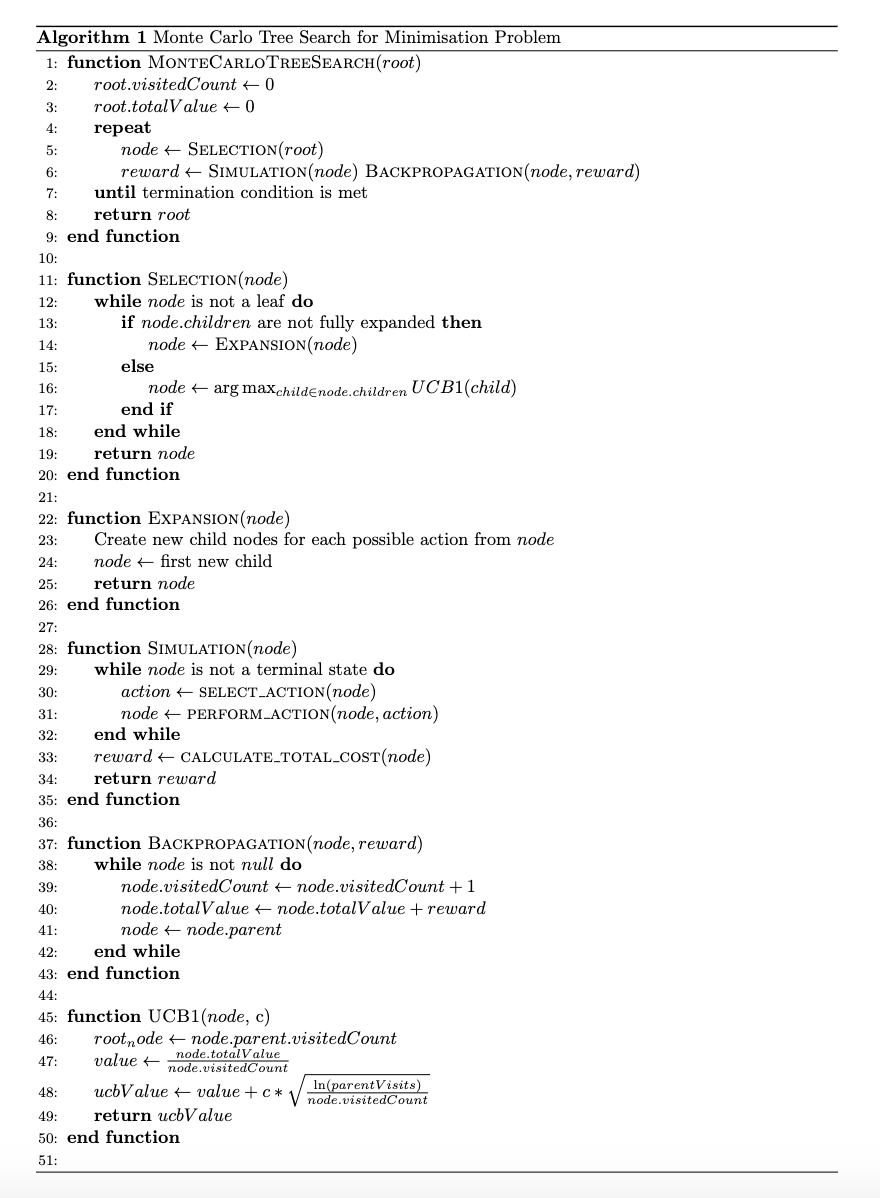
\includegraphics[width=1\textwidth]{Figures/Pseudo code.png}
    \end{figure}
\newpage
\subsection{Different policies}
\subsubsection{Selection policy}
Our selection policy is based on 
\subsubsection{Simulation policy}

